% !TeX root = ../libro.tex
% !TeX encoding = utf8

\chapter{Resultados principales}

\section{Enunciados}
	\begin{teora}
		Toda variedad topológica 2-dimensional tiene una estructura diferenciable.
	\end{teora}

	\begin{teorb}
		Todo homeomorfismo entre variedades diferenciables 2-dimensionales es isotópico a un difeomorfismo.
	\end{teorb}
	
	Suponiendo ciertos los teoremas anteriores, es directa la obtención del siguiente resultado, ya que por A tenemos que toda variedad topológica 2-dimensional tiene una estructura diferenciable y por B sabemos que es única salvo difeomorfismos:
	
	\begin{corolario} (Teorema clásico de Munkres)
		Toda variedad topológica 2-dimensional tiene una única estructura diferenciable salvo difeomorfismos.
	\end{corolario}

\section{Demostración del Teorema A}

	\begin{teora}
		Toda variedad topológica tiene una estructura diferenciable.
	\end{teora}
	\begin{proof}[Demostración]
		Sea S una variedad topológica, podemos coger un atlas $\{h_i | 1\leq i\leq N\}$ con $N \in \N$ si es finito o $N = \infty$ si no lo es. Vamos a construir por inducción una estuctura diferenciable en el conjunto $U_n = \cup_{i\leq n}h_i(\R^2)$, que por ser un sistema coordenado su límite debe de ser S, probando así el resultado. Cabe destacar que cada $U_i$ contiene a todos los anteriores. \\
		\\ La inducción empieza tomando una carta cualquiera del sistema, $U_1=h_1(\R^2)$ por ejemplo. Si se considera la variedad $U_1$ con el atlas $\{h_1\}$ entonces $h_1$ es diferenciable para ésta de forma trivial (se compone con la inversa y queda la identidad en $\R^2$).\\
		\\ Una vez arrancada la inducción, suponiendo cierto para el paso $n-1$ vamos a extender la diferenciabilidad de $U_{n-1}$ a $U_n$. Sea la carta $h_n$, tomamos entonces $W=h_n^{-1}(U_{n-1})=h_n^{-1}(U_{n-1}\cap h_n(\R^2))$, que es un abierto de $\R^2$ por ser $h_n$ continua. \\
		\\ Tenemos $W\subset \R^2$ abierto, por el \textbf{Hecho 1} sabemos que existe una triangulación geométrica suya y al ir acercándose a la frontera topológica los triángulos convergen a puntos. Queremos aplicar el ``Teorema de alisamiento de asas'' en los vértices de los triángulos, seguidamente en los lados y finalmente en el interior de cada uno (aplicar los 3 apartados del teorema de forma consecutiva), pero para ello es necesario partir de un embebimiento de $\R^2$:
		\begin{enumerate}
			\item Para todos y cada uno de los vértices de la triangulación elegimos una bola $B(p, \epsilon_p) \subset W$ cuyos cierres topológicos en $\R^2$ no se corten mutuamente. $B(p,\varepsilon _p)$ es abierto y queremos obtener $\widehat{h}$ diferenciable entorno a $p$. \\
			\newpage
			\begin{figure}[h]
  				\centering
  				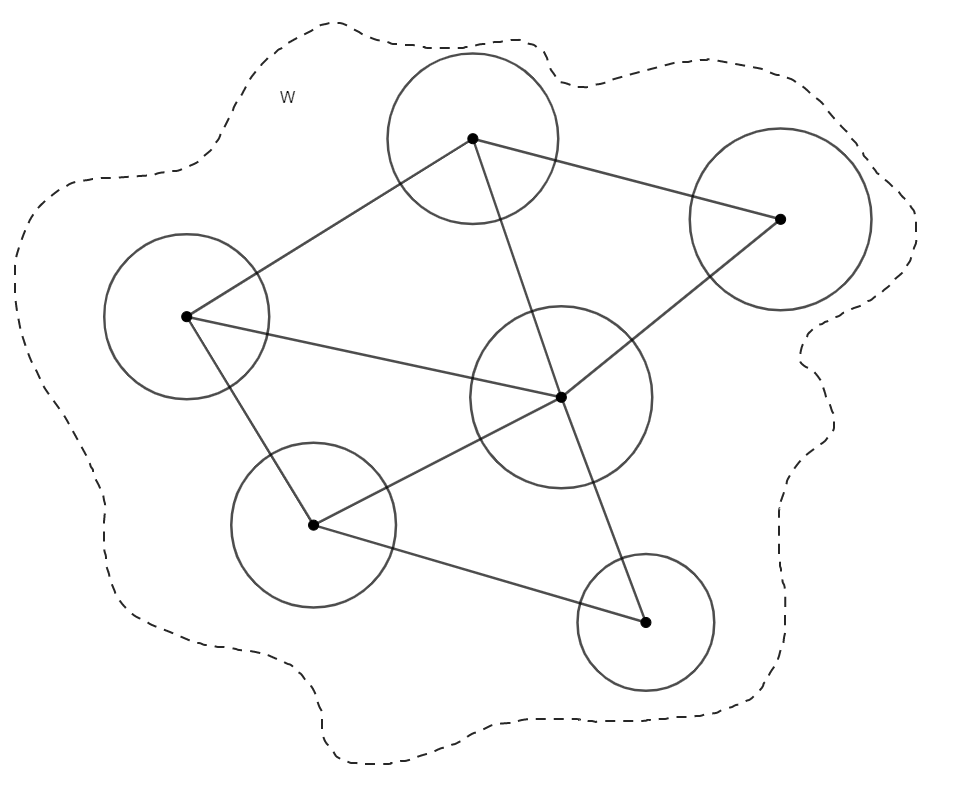
\includegraphics[width=0.5\textwidth]{triangulacion_bolas}
  				\caption{$B(p, \epsilon_p)$ para cada vértice.}
  				\label{fig:triangulacion_bolas}
			\end{figure}
			Podemos aplicar el Corolario del apartado 1 del Teorema de Alisamiento de Asas ya que cumplimos todas las hipótesis necesarias. Así obtenemos una $\widehat{h}$ isotópica a $h$, que es diferenciable en $O_p$ entorno abierto de $p$ y además queda fija fuera de otro entorno un poco mayor $O_p'\supset O_p$, con $O'_p\subset B(p, \epsilon_p) $.\\
			\\ De manera acumulativa, este procedimiento se puede realizar simultáneamente en todos los vértices $p$ en la triangulación de $W$. Esto prueba que $h_n: \R^2 \rightarrow h_n(\R^2)$ es isotópica a un homeomorfismo $\widehat{h}_n: \R^2 \rightarrow h_n(\R^2)$ que es diferenciable, como aplicación sobre la superficie diferenciable $U_{n-1}$, en un entorno $O_p \subset W$ alrededor de cada vértice $p$ de la triangulación de $W$. Además la isotopía coincide con $h_n$ fuera de entornos $O'_p \subset W$ mayores que $O_p$ para cada $p$, disjuntos $2$ a $2$.\\
			\begin{figure}[h]
  				\centering
  				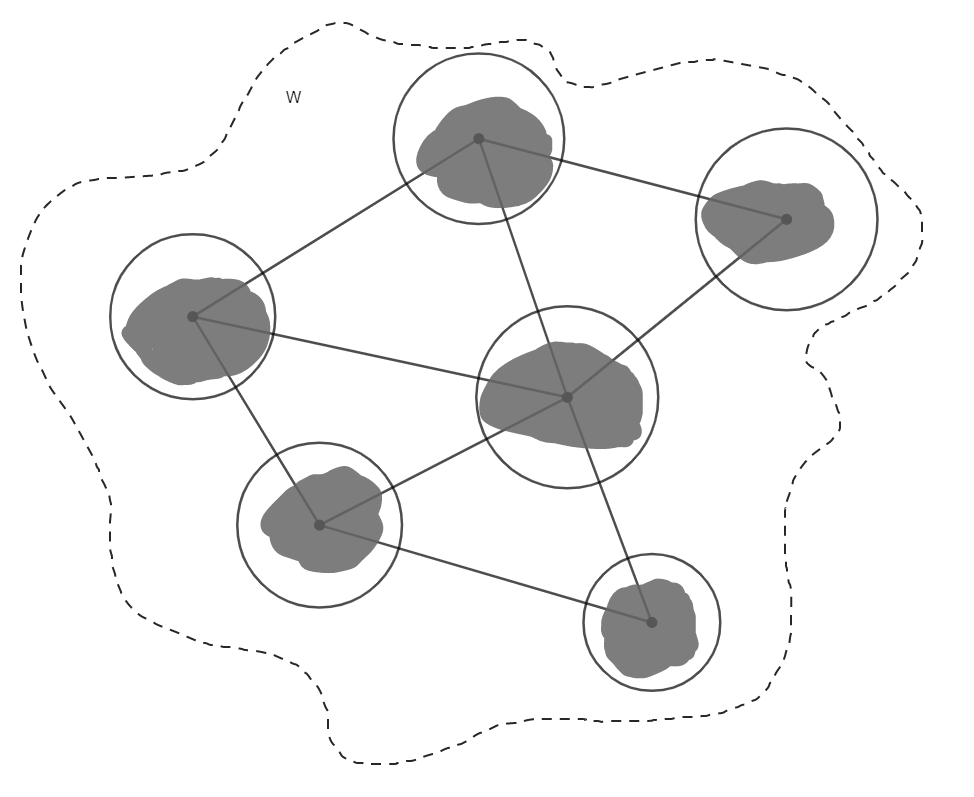
\includegraphics[width=0.5\textwidth]{triangulacion_bolas_suavizado}
  				\caption{$O_p$ para cada vértice.}
  				\label{fig:triangulacion_bolas_suavizado}
			\end{figure}

			\item Tenemos por el paso anterior un $h_n: \R^2 \rightarrow h_n(\R^2)$ isotópico al original en las condiciones explicadas, y que es diferenciable como aplicación $W \rightarrow U_{n-1}$ entorno a los vértices de la triangulación de $W$. Queremos utilizar el apartado $2$ del Teorema de Alisamiento de Asas para generar otra isotopía que nos lleve $h_n$ a otro homeomorfismo (al que le daremos el mismo nombre) cuya restricción a $W \rightarrow U_{n-1}$ sea diferenciable además entorno a los lados de la triangulación anterior, coincidiendo con el $h_n$ original fuera de un entorno del $1$-esqueleto de esa triangulación.\\
			\\ Para ello, consideramos para cada lado $l$ de la triangulación de $W$ un subconjunto $R_l$ (rectángulo) dentro de $W$ que sea difeomorfo a $D^1 \times \R$, cumpliendo:
				\begin{enumerate}
					\item $R_l$ corta a $l$ en un segmento compacto y es disjunto con cualquier otro lado de la triangulación de $W$. En particular, $R_l$ no contiene ningún vértice de la triangulación de $W$.
					\item Si $p_1$ y $p_2$ son los vértices extremos de $l$, una componente del borde de $R_l$ está contenida en $O_{p_1}$ y la otra en $O_{p_2}$, es decir, $h_n$ es diferenciable en 2 componentes de $\partial R_l$.
					\item Los cierres de los rectángulos $R_l$ en $\R^2$ son disjuntos $2$ a $2$ y están contenidos en $W$.
				\end{enumerate}
			\begin{figure}[h]
  				\centering
  				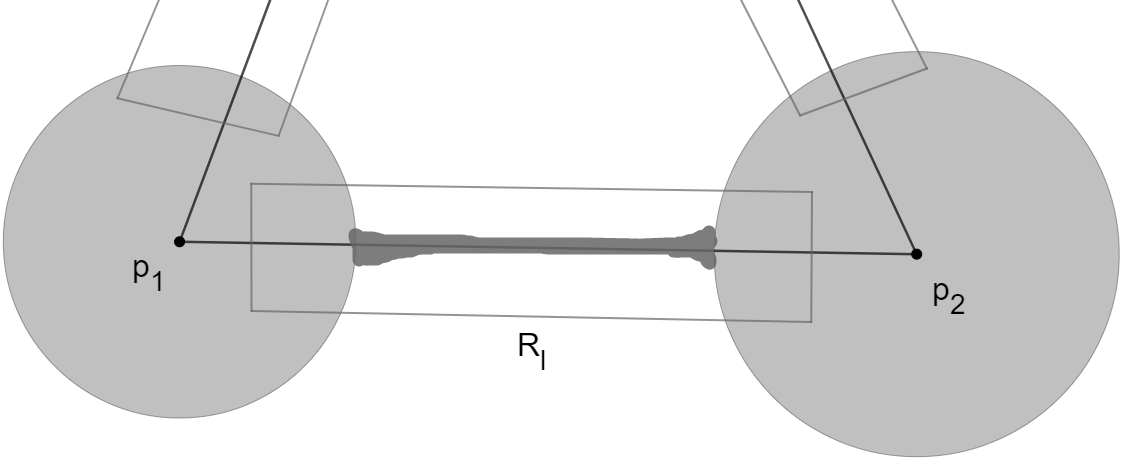
\includegraphics[width=0.5\textwidth]{triangulacion_rectangulos_suavizado}
  				\caption{Entorno de $l$ donde $h_n$ es diferenciable.}
  				\label{fig:triangulacion_rectangulos_suavizado}
			\end{figure}

			Ahora es evidente como en el apartado $2$ del Teorema de Alisamiento de Asas nos produce la isotopía deseada realizando el trabajo simultáneamente en todos los rectángulos $R_l$, generando el nuevo $h_n:\R^2 \rightarrow h_n(\R^2)$ deseado.
			\begin{figure}[h]
  				\centering
  				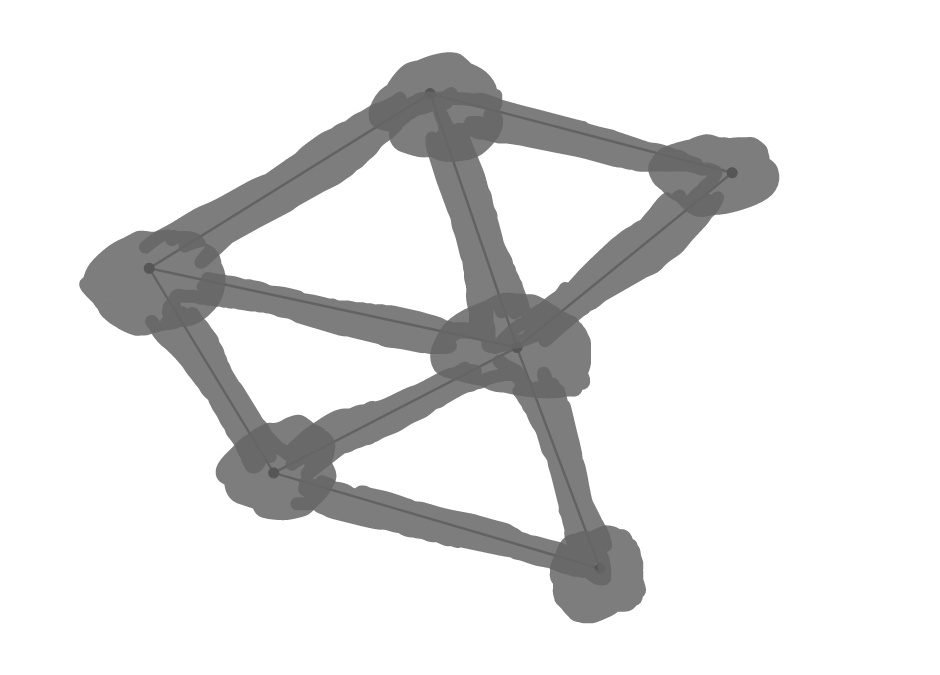
\includegraphics[width=0.45\textwidth]{triangulacion_aristas}
  				\caption{Entorno del $1$-esqueleto donde $h_n$ es diferenciable.}
  				\label{fig:triangulacion_aristas}
			\end{figure}

			\item El tercer paso es similar a los anteriores, pero ahora usando el apartado $3$ del Teorema de Alisamiento de Asas. Lo que hacemos en considerar para cada triángulo $T$ de la triangulación de $W$ un dominio de Jordan $D_T$ satisfaciendo:
			\begin{enumerate}
				\item $D_T \subset \mathring{T}$.
				\item $h_n:W \rightarrow U_{n-1}$ es diferenciable sobre $T-\mathring{D_T}$.
				\item Los $D_T$ son disjuntos dos a dos.
			\end{enumerate}
			
			Aplicando el Teorema de Carathéodory obtenemos que es difeomorfo a la bola unidad y por tanto podemos proceder de manera similar a los apartados anteriores. \\
			\\ A continuación producimos otra isotopía que nos lleve el $h_n$ generado en el apartado $2$ a otro homeomorfismo (al que daremos el mismo nombre) cuya restricción $W \rightarrow U_{n-1}$ sea diferenciable sobre $D_T$, coincidiendo en cada instante con la $h_n$ anterior en un entorno de $\partial D_T$ y de hecho fuera de $D_T$, para cada triángulo $T$. Esto concluiría la prueba. \\
			\\ Para probar la existencia de $D_T$ vamos a definir la curva de Jordan cuyo interior es de forma trivial un dominio de Jordan, que será dicho $D_T$. La curva debe ser diferenciable, cerrada y simple, que es la caracterización de una curva de Jordan. Reducimos el problema a buscar dicha curva para el entorno tubular de un triángulo equilátero, ya que es difeomorfo al de un triángulo cualquiera. Podemos simplificarlo más aportando únicamente una curva no cerrada cuyos extremos se puedan pegar consecutivamente, siendo infinitamente derivable en los puntos donde se unen.\\
			\\ Haciendo uso de una función meseta $f$ que vale $0$ en $\mathbb{R}^-$ y $1$ a partir de $\epsilon > 0$, si tomamos $g(x)=tg(\frac{\pi}{3})xf(x)$ en el intervalo $[-1,\epsilon]$, tenemos que $g(-1)=0$ y $g(\epsilon)=tg(\frac{\pi}{3})\epsilon$  al igual que sus derivadas, por lo que si vamos alternando $g(x)$ y $g(-x)$ mediante rotaciones y traslaciones, tendremos una curva $\alpha$ diferenciable (suavización del triángulo equilátero). \\
			%\newpage
			\begin{figure}[h]
  				\centering
  				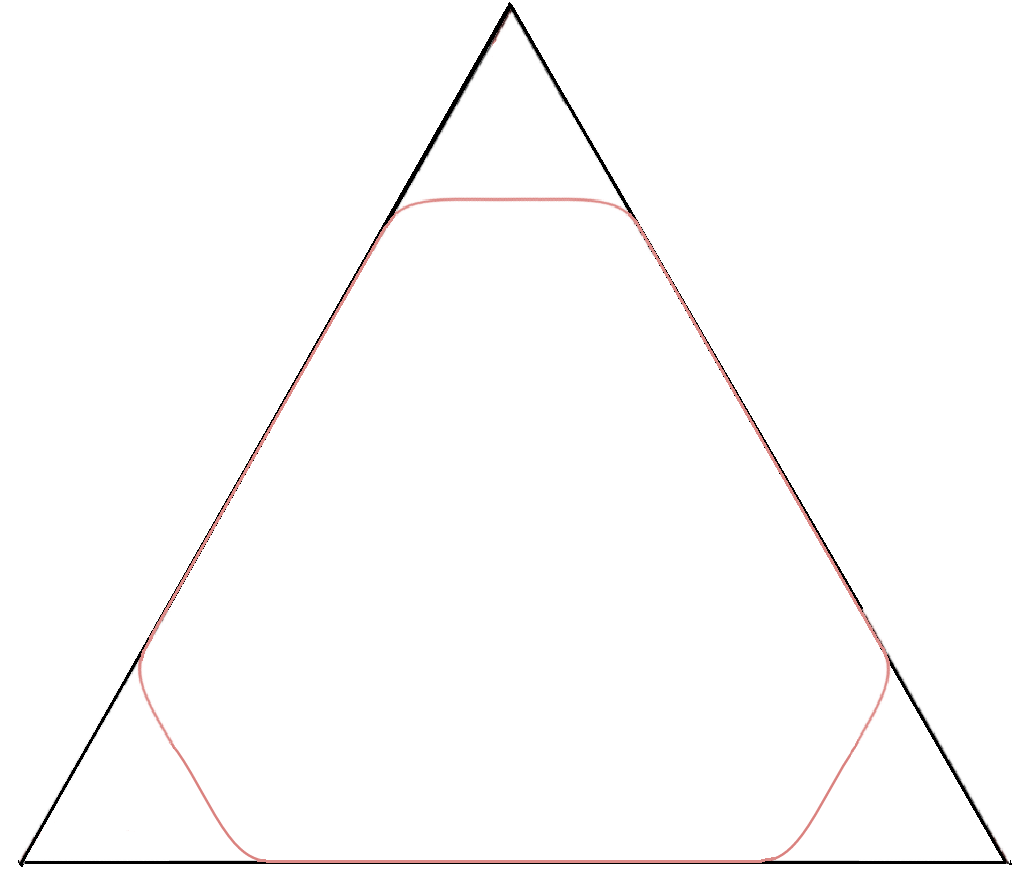
\includegraphics[width=0.5\textwidth]{triangulo_suavizado}
  				\caption{Curva de Jordan cercana al triángulo}
  				\label{fig:triangulo_suavizado}
			\end{figure}
			\\ Se puede observar que es válido $\forall \epsilon > 0$ y que al hacer tender $\epsilon$ a $0$, la curva será el propio triángulo equilátero. Es por ello que podemos tomar el $\epsilon$ lo suficientemente pequeño como para que la curva $\alpha$ quepa en el entorno tubular y siga siendo una curva de Jordan. Como exigimos que $D_T \subset \mathring{T}$ podemos aplicar a la curva un factor de escala para así no contener ningún punto del borde del triángulo $T$. Además, de forma evidente obtenemos que los dominos $D_T$ son disjuntos $2$ a $2$.
		\end{enumerate}

		Todas las isotopías de los pasos anteriores coinciden por extensión continua con el homeomorfismo $h_n:\R^2 \rightarrow h_n(\R^2)$ original en la frontera de $W$ en $\R^2$ por construcción, ya que el diámetro de los triángulos en $W$ tiende a $0$ al acercarnos a la frontera. Por tanto pueden ser extendidas como isotopías de $\R^2 \rightarrow h(\R^2)$ coincidentes con $h_n$ en $\R^2 - W$. \\
		\\ Como conclusión, el homeomorfismo $h_n:\R^2 \rightarrow h_n(\R^2)$ resultante es compatible con la estructura diferenciable en $U_{n-1}$ y junto con $h_1$, $\ldots$, $h_{n-1}$, nos define una estructura diferenciable sobre $U_n$. Esto cierra la inducción y prueba el teorema. \\
	\end{proof}

\section{Demostración del Teorema B}
	\begin{teorb}
		Todo homeomorfismo entre variedades diferenciables 2-dimensionales es isotópico a un difeomorfismo.
	\end{teorb}
	\begin{proof}[Demostración]
		Sea $f: S \rightarrow S'$ homeomorfismo entre variedades diferenciales 2-dimensionales, se puede utilizar el \textbf{Hecho 2}, que nos aporta una triangulación diferenciable de $S$. Por definición de triangulación diferenciable, tenemos que la aplicación celda $\varphi_n$ es un difeomorfismo. Vamos a proseguir de forma similar a la demostración del Teorema A, pero esta vez la función a isotopar es $g_n = f \circ \varphi_n : \R^2 \rightarrow f(\varphi(\R^2)) \subset S'$ homeomorfismo. Sea $W_n = \varphi_n^{-1}(S) = \varphi_n^{-1}(S \cap \varphi_n(\R^2))$ abierto de $\R^2$, vamos a isotopar $f$ en $3$ etapas:
		\begin{enumerate}
			\item Para todos los vértices de la triangulación de $S$, vistos en $W_n$ mediante $\varphi_n^{-1}$, tomamos una bola $B(p, \epsilon)$ de tal forma que sus cierres no se corten $2$ a $2$ y estén contenidos en $W_n$. Acto seguido podemos proceder de forma idéntica al apartado $1$ de la demostración del Teorema A, obteniendo como resultado un homeomorfismo $\widehat{g}_n : W_n \rightarrow g_n(W_n)$ isotópico a $g_n$, que es diferenciable en un entorno de cada vértice de la triangulación $O_p \subset W_n$, cuyos cierres no se cortan y quedan dentro de $W_n$ y además $\widehat{g}_n$ coincide con $g_n$ en un entorno de cada vértice mayor al anterior (cuyos cierres tampoco se cortan y están contenidos en $W_n$). \\
			\\ Si deshacemos el cambio con $\varphi_n$, obtenemos que $f: \widehat{g} \circ \varphi_n : \varphi_n(W_n) \rightarrow g_n(W_n)$ homeomorfismo es isotópica a $\widehat{f} = \widehat{g} \circ \varphi_n : \varphi_n(W_n) \rightarrow g_n(W_n)$ homeomorfismo, cumpliendo lo descrito pero para $\varphi_n(W_n)$, por ser $\varphi_n$ un difeomorfismo. Como $\widehat{f}$ coincide con $f$ en el borde de $\varphi_n(W_n)$, la isotopía se puede extender a $S \rightarrow S'$. Mantenemos el nombre $f$ para la nueva $\widehat{f}$. \\
			\\ Realizamos de forma incremental este proceso, hasta conseguir una isotopía a una función que sea diferenciable en un entorno de todos los vértices de la triangulación de $S$ que además queda fija en un entorno mayor (cuyos cierres no se cortan).
			\item Para todo lado $l$ de la triangulación en $W_n$ definimos un entorno $R_l$ que es difeomorfo a un rectángulo, que a su vez es difeomorfo a $D^1 \times \R$, para así poder aplicar el apartado $2$ del Teorema de Alisamiento de Asas. Para ello debe cumplir:
			\begin{enumerate}
				\item $R_l$ corta a $l$ en una curva compacta y es disjunto con cualquier otro lado de la triangulación diferenciable. En particular $R_l$ no contiene ningún vértice de la triangulación en $W_n$.
				\item Si $p_1$ y $p_2$ son los vértices extremos de $l$, una componente del borde está contenida en $O_{p_1}$ y otra en $O_{p_2}$, con $O_p$ entorno de $p$ donde es diferenciable $g_n$, es decir, defimimos $R_l$ de manera que $g_n$ sea diferenciable en $2$ componentes de su borde ($\partial R_l$).
				\item Los cierres de los $R_l$ en $\R^2$ son disjuntos $2$ a $2$ y están contenidos en $W_n$.
			\end{enumerate}
			Estamos en las condiciones necesarias para aplicar el apartado $2$ del Teorema de Alisamiento de Asas, dando lugar a una isotopía a $\widehat{g} : W_n \rightarrow g(W_n)$ homemomorfismo diferenciable en un entorno de cada lado de la triangulación en $W_n$ que coincide con $g$ fuera de un entorno mayor al anterior. Procedemos de igual forma que en el apartado $1$ de esta demostración, obteniendo una isotopía de $f$ a $\widehat{f} : S \rightarrow S'$ homeomorfismo diferenciable en un entorno de cada lado de la triangulación diferenciable de $S$, que coincide con $f$ fuera de un entorno mayor que el anterior.
			\item En este último apartado queremos aplicar el punto $3$ del Teorema de Alisamiento de Asas. Como la triangulación de $S$ es diferenciable, sabemos que el interior de cada triángulo es difeomorfo al disco unidad de $\R^2$, por lo que para utilizar un dominio de Jordan $D_T$ para cada $T$ triángulo de la triangulación de $W_n$ de forma que no se corten $2$ a $2$, tomamos un conjunto más pequeño que el interior del triángulo (se puede tomar el mismo conjunto pero multiplicado por un factor de escala ligeramente menor que $1$).\\
			\\ Tenemos que $g_n$ es diferenciable en un entorno de $\partial D_T$ y coincide con la $g$ original fuera de un entorno del borde mayor que el anterior. De igual forma que en el apartado $3$ de la demostración del Teorema B obtenemos una isotopía de $g$ a $\widehat{g} : W_n \rightarrow g_n(W_n)$ homemorfismo que es diferenciable en la triangulación de $W_n$ (en los vértices, los lados y en el interior de cada triángulo). Siguiendo el esquema de los apartados anteriores obtenemos que $f$ es isotópica a $\widehat{f}: S \rightarrow S'$ homeomorfismo diferenciable en toda la triangulación diferenciable de $S$ (vértices, lados e interiores). Como consecuencia $\widehat{f}$ es, de forma natural, un difeomormismo, concluyendo así la prueba.
		\end{enumerate}
	\end{proof}
\endinput
%------------------------------------------------------------------------------------
% FIN DEL CAPÍTULO. 
%------------------------------------------------------------------------------------
